\documentclass[border=4pt]{standalone}
\usepackage{tikz}

\begin{document}
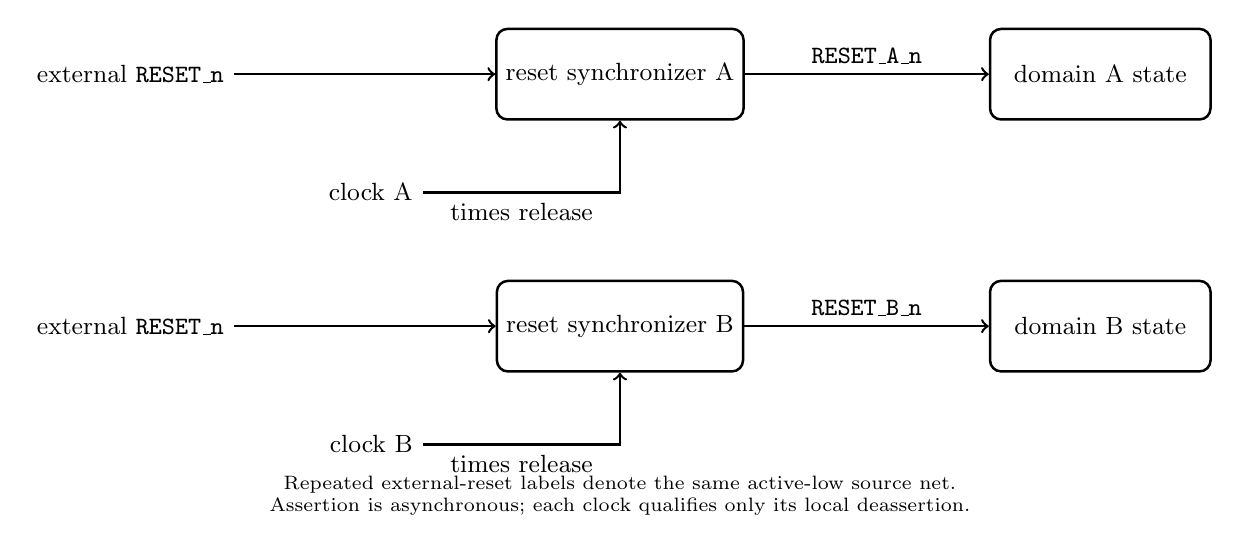
\begin{tikzpicture}[x=1cm,y=1cm,font=\small,line width=0.9pt,
  block/.style={draw,rounded corners=4pt,minimum width=2.8cm,
    minimum height=1.15cm,align=center}]
  \node[block] (RA) at (5.5,4.8) {reset synchronizer A};
  \node[block] (DA) at (11.6,4.8) {domain A state};
  \node[block] (RB) at (5.5,1.6) {reset synchronizer B};
  \node[block] (DB) at (11.6,1.6) {domain B state};

  \coordinate (R1) at (0.6,4.8);
  \coordinate (R2) at (0.6,1.6);
  \coordinate (CA) at (3.0,3.3);
  \coordinate (CB) at (3.0,0.1);

  \draw[->] (R1) node[left] {external \texttt{RESET\_n}} -- (RA.west);
  \draw[->] (R2) node[left] {external \texttt{RESET\_n}} -- (RB.west);
  \draw[->] (CA) node[left] {clock A} -| (RA.south)
    node[pos=0.25,below] {times release};
  \draw[->] (CB) node[left] {clock B} -| (RB.south)
    node[pos=0.25,below] {times release};
  \draw[->] (RA.east) -- (DA.west)
    node[midway,above] {\texttt{RESET\_A\_n}};
  \draw[->] (RB.east) -- (DB.west)
    node[midway,above] {\texttt{RESET\_B\_n}};

  \node[align=center,font=\scriptsize] at (5.5,-0.55)
    {Repeated external-reset labels denote the same active-low source net.\\
     Assertion is asynchronous; each clock qualifies only its local deassertion.};
\end{tikzpicture}
\end{document}
